% Created 2016-08-17 Wed 14:38
\documentclass[tikz]{standalone}

\usepackage[utf8]{inputenc}
\usepackage[T1]{fontenc}
\usepackage{helvet}
\usepackage{../../templates/msc}

\renewcommand{\familydefault}{\sfdefault}

\tikzset{
every picture/.style={
line width=1pt
}}

\usepackage{tikz}
\author{Holger Karl}
\date{\today}
\title{}


\usetikzlibrary{arrows,automata}

\begin{document}

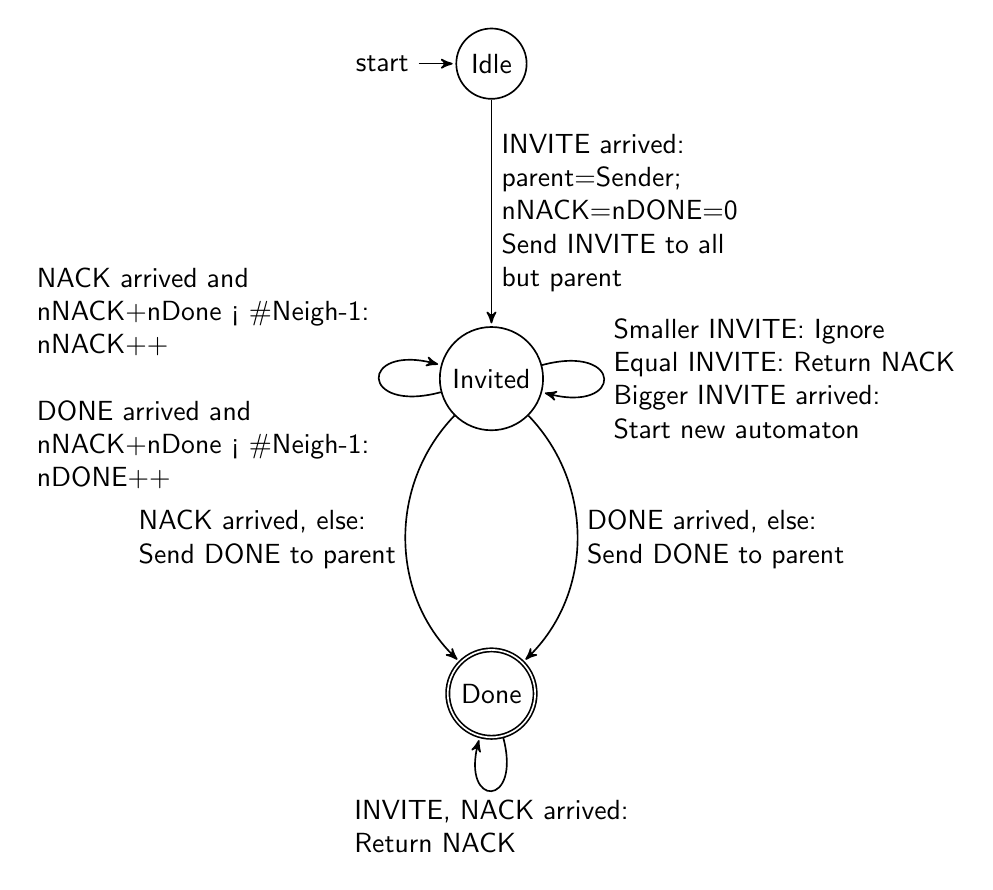
\begin{tikzpicture}[->,>=stealth',shorten >=1pt,auto,node distance=4cm, semithick]

\node[initial, state] (idle) {Idle}; 
\node[state] (invited) [below of=idle] {Invited}; 
\node[state, accepting] (done) [below of=invited] {Done}; 

\path (idle) edge node[align=left] {INVITE arrived: \\ parent=Sender; \\nNACK=nDONE=0 \\ Send INVITE to all \\but parent} (invited)
(invited) edge [loop left] node [align=left] {NACK arrived and \\ nNACK+nDone < \#Neigh-1:\\nNACK++  \\ \\
DONE arrived and \\ nNACK+nDone < \#Neigh-1:\\nDONE++ 
} (invited) 
(invited) edge [loop right] node [align=left]{Smaller INVITE: Ignore \\ 
 Equal INVITE: Return NACK\\ 
Bigger INVITE arrived:\\
Start new automaton}
 (invited) edge [bend right=45, auto,swap] node [align=left] {NACK arrived, else: \\ Send DONE to parent} (done) 
 (invited) edge [bend left=45, auto] node [align=left]  {DONE arrived, else: \\  Send DONE to parent} (done) 
(done) edge[loop below] node[align=left] {INVITE, NACK arrived:\\ Return NACK}  (done)
;
\end{tikzpicture}


\end{document}